\part{Integer and Combinatorial Programming}
	\chapter{Formulation}
		\section{Typical Problems}

		\section{Integer Programming Formulation Skills}
			\subsection{A Variable Taking Discontinuous Values}
				In algebraic notation: 
				\begin{equation}
					x = 0,\quad \text{or} \quad l\le x \le u 
				\end{equation}
				Modeling:
				\begin{align}
					& x \le uy \\
					& x \ge ly  \\
					& y \in \{0, 1\} 
				\end{align}
				where
				\begin{equation}y=\begin{cases}0, & \text{if }x=0 \\ 1, & \text{if } l\le x \le u\end{cases} \end{equation}
					
			\subsection{Fixed Costs}
				In algebraic notation: 
				\begin{equation}
					C(x) = \begin{cases} 0 & \text{for } x=0 \\ k + cx & \text{for } x > 0 \end{cases} 
				\end{equation}
				Modeling:
				\begin{align}
					& C^*(x, y) = ky+cx\\
					& x \le My  \\
					& x \ge 0 \\
					& y \in \{0, 1\} 
				\end{align}
				where
				\begin{equation}y=\begin{cases}0, & \text{if }x=0 \\ 1, & \text{if }x\ge 0\end{cases} \end{equation}
			
			\subsection{Either-or Constraints}
				In algebraic notation: 
				\begin{equation}
					\sum_{j\in J} a_{1j} x_j \le b_1 \text{ or } \sum_{j\in J} a_{2j} x_j \le b_2 
				\end{equation}
				Modeling:
				\begin{align}
					& \sum_{j\in J} a_{1j} x_j \le b_1 + M_1y  \\
					& \sum_{j\in J} a_{2j} x_j \le b_2 + M_1(1-y)  \\
					& y \in \{0, 1\} 
				\end{align}
				where
				\begin{equation}y=\begin{cases}0, & \text{if }\sum_{j\in J} a_{1j} x_j \le b_1 \\ 1, & \text{if } \sum_{j\in J} a_{2j} x_j \le b_2\end{cases} \end{equation}
				Notice that the sign before $M$ is determined by the inequality $\ge$ or $\le$, if it is \lq\lq{}$\ge$\rq\rq{}, use \lq\lq{}$-$\rq\rq{}, if it \lq\lq{}$\le$\rq\rq{}, use \lq\lq{}+\rq\rq{}.
			
			\subsection{Conditional Constraints}
				If constraint A is satisfied, then constraint B must also be satisfied
				\begin{equation}
					\text{If} \quad \sum_{j\in J} a_{1j} x_j \le b_1 \text{ then } \sum_{j\in J} a_{2j} x_j \le b_2 
				\end{equation}
				The key part is to find the opposite of the first condition. We are using $A\Rightarrow B \Leftrightarrow \neg B \Rightarrow \neg A$\\
				Therefore it is equivalent to
				\begin{equation}
					\sum_{j\in J} a_{1j} x_j > b_1 \text{ or } \sum_{j\in J} a_{2j} x_j \le b_2 
				\end{equation}
				Furthermore, it is equivalent to
				\begin{equation}
					\sum_{j\in J} a_{1j} x_j \ge b_1 + \epsilon \text{ or } \sum_{j\in J} a_{2j} x_j \le b_2 
				\end{equation}
				Where $\epsilon$ is a very small positive number.\\
				Modeling:
				\begin{align}
					& \sum_{j\in J} a_{1j} x_j \ge b_1 + \epsilon -  M_2y  \\
					& \sum_{j\in J} a_{2j} x_j \le b_2 + M_2(1-y)  \\
					& y \in \{0, 1\} 
				\end{align}	
			
			\subsection{Special Ordered Sets}
				\framebox{\textbf{SOS1 Description}} Out of a set of yes-no decisions, at most one decision variable can be yes. \
				\begin{align}
					x_1=1,x_2=x_3&=\dots=x_n=0  \\
					&\text{or}  \\
					x_2=1, x_1=x_3&=\dots=x_n=0  \\
					&\text{or ...} 
				\end{align} 
				Modeling:
				\begin{equation} \sum_{i} x_i = 1, \quad i \in N \end{equation}
				\framebox{\textbf{SOS2 Description 1}} Out of a set of binary variables, at most two variables can be nonzero. In addition, the two variables must be adjacent to each other in a fixed order list.\\
				Modeling:
				If $x_1, x_2, ... , x_n$ is a SOS2, then
				\begin{align}
					& \sum_{i=1}^{n} x_i \le 2  \\
					& x_i + x_j \le 1, \forall i \in \{1, 2,..., n\}, j \in \{i+2, i+3, ..., n\}  \\
					&x_i \in \{0, 1\}
				\end{align}
				\framebox{\textbf{SOS2 Description 2}} There is another type of definition, that is out of a set of nonnegative variables \textbf{not binary here}, at most two variables can be nonzero. In addition, the two variables must be adjacent to each other in a fixed order list. All variables summing to 1.\\
				This definition of SOS2 is used in the following section \textit{Piecewise Linear Formulations}\\
								
			\subsection{Piecewise Linear Formulations}
				The objective function is a sequence of line segments, e.g. $y=f(x), $ consists $k-1$ linear segments going through $k$ given points $(x_1, y_1), (x_2, y_2), ... ,(x_k, y_k)$.\\
				Denote 
				\begin{equation}d_i=\begin{cases}1, & x\in (x_i, x_{i+1})\\0, & \text{otherwise} \end{cases}\end{equation}
				Then the objective function is
				\begin{equation}\sum_{i \in \{1, 2, ..., k-1\}} y = d_if_i(x) \end{equation} 
				Modeling: Given that objective function as a piecewise linear formulation, we can have these constraints\\
				\begin{align}
					&\sum_{i \in \{1, 2, ..., k-1\}} d_i =1  \\
					&d_i \in \{0, 1\}, i \in \{1, 2, ..., k-1\}  \\
					& x = \sum_{i \in \{1, 2, ..., k\}} w_i x_i  \\
					& y = \sum_{i \in \{1, 2, ..., k\}} w_i y_i  \\
					& w_1 \le d_1  \\
					& w_i \le d_{i-1} + d{i}, i \in \{2, 3, ..., k-1\}  \\
					& w_k \le d_{k-1} 
				\end{align}
				In this case, $ w_i \in SOS2$ (second definition)		
									
			\subsection{Conditional Binary Variables}
				Choose at most $n$ binary variable to be 1 out of  $x_1, x_2, ... x_m, m\ge n$. If $n=1$ then it is SOS1.\\
				Modeling:
				\begin{equation}
					\sum_{k\in \{1,2,...,m\}} x_k \le n
				\end{equation}
				Choose exactly $n$ binary variable to be 1 out of  $x_1, x_2, ... x_m, m\ge n$\\
				Modeling:
				\begin{equation}
					\sum_{k\in \{1,2,...,m\}} x_k = n
				\end{equation}
				Choose $x_j$ only if $x_k = 1$\\
				Modeling:
				\begin{equation}x_j = x_k  \end{equation}
				\lq\lq{}and\rq\rq{} condition, iff $x_1, x_2, ... , x_m =1$ then $y=1$\\
				Modeling:
				\begin{align}
					& y \le x_i, i\in \{1, 2, ..., m\}  \\
					& y \ge \sum_{i \in \{1, 2, ..., m\}} x_i - (m - 1) 
				\end{align}

			\subsection{Elimination of Products of Variables}
				For variables $x_1$ and $x_2$,
				\begin{equation}y = x_1 x_2\end{equation}
				Modeling: If $x_1, x_2$ are binary, it is the same as \lq\lq{}and\rq\rq{} condition of binary variables.\\
				If $x_1$ is binary, while $x_2$ is continuous and $0 \le x_2 \le u$, then
				\begin{align}
					y &\le ux_1  \\
					y &\le x_2  \\
					y &\ge x_2 - u(1- x_1)  \\
					y &\ge 0 
				\end{align}
				If both $x_1$ and $x_2$ are continuous, it is non-linear, we can use Piecewise linear formulation to simulate.

	\chapter{Polyhedral Analysis}
		\section{Polyhedral and Dimension}  
			\subsection{Polyhedral, Hyperplanes and Half-spaces}
				- A \textbf{polyhedron} is a set of the form $\{x\in \mathbb{R}^n|Ax\le b\}=\{x \in \mathbb{R}^n | a^ix\le b^i, \forall i \in M\}$, where $A \in \mathbb{R}^{m\times n}$ and $b \in \mathbb{R}^m$\\
				- A polyhedron $P \subset \mathbb{R}^n$ is \textbf{bounded} if there exists a constant $K$ such that $|x_i|<K, \forall x \in P, \forall i \in [1, n]$, in this case the polyhedron is call \textbf{polytopes}\\
				- The lower-bound of $K$ is called \textbf{diagonal} denoted by $d$\\
				
			\subsection{Open, Close Sets: boundary and interior}
				- Denote $N_\epsilon = \{y\in \mathbb{R}^n|\lVert y-x\rVert < \epsilon \}$ as the \textbf{neighborhood} of $x\in \mathbb{R}^n$\\						
				- Given $S\subseteq \mathbb{R}^n$, x belongs to the \textbf{interior} of $S$, denoted by $int(S)$ if there is $\epsilon > 0$ such that $N_\epsilon(x) \le S$\\
				- $S$ is said to be an \textbf{open set} iff $S=int(S)$\\
				- $x$ belongs to the \textbf{boundary} $\partial S$ if $\forall \epsilon >0$, $N_\epsilon(x)$ contains at least one point in $S$ and a point not in $S$\\
				- $x\in S$ belongs to the \textbf{closure} of $S$, denoted $cl(s)$ if $\forall \epsilon > 0$, $N_\epsilon(x) \cap S = \emptyset$
				- $S$ is called \textbf{closed} iff $S=cl(S)$\\
				- In IP, LP, MIP, etc. we always work with close set. No \lq\lq{}$<$\rq\rq{} or \lq\lq{}$>$\rq\rq{}
				
			\subsection{Hyperplane and half-space}
				- A \textbf{hyperplane} is $\{x\in \mathbb{R}^n|a^Tx=b\}$\\
				- A \textbf{half-space} is  $\{x\in \mathbb{R}^n|a^Tx\le b\}$
				
			\subsection{Dimension of Polyhedral}
				- A polyhedron $P$ is \textbf{dimension} $k$, denoted $dim(P)=k$, if the maximum number of affinely independent points in $P$ is $k+1$\\
				- A polyhedron $P\subseteq \mathbb{R}^n$ is \textbf{full-dimensional} if $dim(P) = n$\\
				- Let:\\
				\indent - $M=\{1, 2, ..., m\}$\\
				\indent - $M^= = \{i \in M | a_ix=b_i, \forall x \in P\}$, i.e. the equality set\\
				\indent - $M^\le = M \setminus  M^=$, i.e. the inequality set\\
				- Let $(A^=, b^=)$, $(A^\le, b^\le)$ be the corresponding rows of $(A, b)$\\
				- If $P\subseteq \mathbb{R}^n$, then $dim(P) = n - rank(A^=, b^=)$\\
				- To proof a constraint $(A^=, b^=)$ is an equality constraint, we need to proof all point in the closure of $P$ satisfied the constraint, to proof it is not an equality constraint, we need to find one point that is not in the hyperplane.
			
			\subsection{Dimension and Rank}
				- $x\in P$ is called an \textbf{inner point} of $P$ if $a^ix < b_i, \forall i \in M^\le$\\
				- $x\in P$ is called an \textbf{interior point} of $P$ if $a^ix<b_i, \forall i \in M$\\
				- Every nonempty polyhedron has at least one inner point\\
				- A polyhedron has an interior point iff $P$ is full-dimensional, i.e., there is no equality constraint
		
		\section{Face and Facet}
			\subsection{Valid Inequalities and Faces}
				- The inequality denoted by $(\pi, \pi_o)$ is called a \textbf{valid inequality} for $P$ if $\pi x \le \pi_0, \forall x \in P$\\
				- Note that $(\pi, \pi_0)$ is a valid inequality iff $P$ lies in the half-space $\{x\in \mathbb{R}^n|Ax\le b\}$\\
				\begin{figure}[h!]
				\centering
				\begin{tikzpicture}[scale=0.4]
					\draw (0,0) -- (3, -0.4) -- (3.3, 4.1) -- (-0.2, 4.1) -- (0, 0);
					\draw (-2, 2) -- (2, -2);
					\draw (4.9, 4.1) -- (-1.8, 4.1);
					\draw (4, 1) -- (2, 6);
					\draw [arrow] (-1.8, 4.1) -> (-1.8, 3.3);
					\draw [arrow] (4.9, 4.1) -> (4.9, 3.3);
					\draw [arrow] (-2, 2) -> (-1, 3);
					\draw [arrow] (2, -2) -> (3, -1);
					\draw [arrow] (4, 1) -> (3, 0.6);
					\draw [arrow] (2, 6) -> (1, 5.6);
					\node at (1, -1) [left] {valid inequality};
					\node at (4.9, 4) [right] {valid inequality (induce a facet)};
					\node at (2, 6) [right] {invalid inequality};
				\end{tikzpicture}
				\caption{Example of valid/invalid inequality}
				\end{figure}\\
				- If $(\pi, \pi_0)$ is a valid inequality for $P$ and $F=\{x\in P|\pi x=x_0\}$, $F$ is called a \textbf{facet} of $P$ and we say that $(\pi, \pi_0)$ \textbf{represents} or \textbf{defines} $F$\\
				- A face is said to be \textbf{proper} if $F\ne \emptyset$ and $F\ne P$\\
				- The face represented by $(\pi, \pi_0)$ is nonempty iff $\max \{\pi x |x\in P\}=\pi_0\}$\\
				- If the face $F$ is nonempty, we say it \textbf{supports} $P$\\
				- Let $P$ be a polyhedron with equality set $M^=$. If 
				\begin{equation}F=\{x\in P | \pi^T x = \pi_0\}  \end{equation}
				is not empty, then $F$ is a polyhedron. Let 
				\begin{equation}M^= \subseteq M_F^=, M_F^{\le}=M \setminus M_F^= \end{equation}
				then 
				\begin{equation}F=\{x | a_i^T x=b_i, \forall i \in M_F^=, a_i^T x \le b_i, \forall i \in M_f^{\le}\} \end{equation}
				
			\subsection{Facet}
				- A face $F$ is said to be a \textbf{facet} of $P$ if $dim(F) = dim(P)-1$\\
				- Facets are all we need to describe polyhedral\\
				- If $F$ is a facet of $P$, then in any description of $P$, there exists some inequality representing $F$\\
				- Every inequality that represents a face that is not a facet is unnecessary in the description of $P$
				- Every full-dimensional polyhedron $P$ has a unique (up to scalar multiplication) representation that consists of one inequality representing each facet of $P$\\
				- If $dim(P) = n-k$ with $k>0$, then $P$ is described by a maximal set of linearly independent rows of $(A^=, b^=)$, as well as one inequality representing each facet of $P$
				
			\subsection{Proving Facet}
				To prove an inequality $\sum_i a_i x_i \le b_i$ is facet inducing for a $D$ dimensional polyhedral, we need to prove there are $D$ affinely independent vectors in $\sum_i a_i x_i = b_i$

			\subsection{Domination}
				$\Pi x\le \Pi_0$ dominates $Mx\le M_0$ if
				\begin{equation}
					\begin{cases}
						\Pi \ge \mu M, \mu > 0\\
						\Pi_0 \le \mu M_0, \mu > 0\\
						(\Pi, \Pi_0) \ne (M, M_0)
					\end{cases}
				\end{equation}

	\chapter{Branch and Bound}
		\section{LP based Branch and Bound}
			\subsection{Idea of Divide and Conquer}
				For each iteration, divide the feasible region of LP into two parts (and an infeasible part), solve the LP in those parts.\\
				\begin{figure}[h!]
					\centering
					\begin{tikzpicture}[scale=0.5]
						\draw [<->] (10, 0) -- (0,0) -- (0,10);
						\draw (0, 8.5) -- (10, 2.5);
						\draw (2, 8) -- (9, 0);
						\draw [dashed] (3,0) -- (3,10);
						\draw [dashed] (4,0) -- (4,10);
						\node at (1.5, 5) {$S_1$};
						\node at (3.5, 4) {$S_2$};
						\node at (5, 3) {$S_3$}; 
					\end{tikzpicture}
					\caption{Divide and Conquer}
				\end{figure}
				In this iteration, the original feasible region have been partition into three parts, where $S_2$ is infeasible for IP because there is not integer point in it. We continue the iteration for $S_1$ and $S_2$. Each partition is suppose to give a new upper bound / lower bound and reduce the infeasible space.\\
				If the temp optimal integer in $S_1$ is larger than the LP relaxation in $S_3$, we can cut $S_3$.\\
				For each iteration, we use dual simple method, for the following two reasons:\\
				\indent - We can process new constraint very fast\\
				\indent - Always gives us a valid bound.\\
				
			\subsection{Relation Between LP Relaxation and IP}
				Let
				\begin{align}
					Z_{IP} &=\max_{x\in S} cx, \quad \text{where } s \text{ is a set of integer solutions} \\
					Z_{LP} &=\max cx, \quad \text{the LP relaxation of IP}  
				\end{align}
				then
				\begin{align}
					Z_{IP} &= \max_{1\le i \le k} \{\max_{x \in S_i} cx \} \\
					\text{iff} \quad S&=\bigcup_{1\le i \le k} S_i 
				\end{align}
				Notice that $S_i$ don\rq{}t need to be disjointed.\\
				\textbf{Important!} (For maximization problem)\\
				\indent - Any feasible solution provides a lower bound $L$, which is also the \textit{Prime Bound}\\
				\begin{equation}\hat{x}\in S \rightarrow Z_{IP}\ge c\hat{x}\end{equation}
				\indent - After branching, solving the LP relaxation over sub-feasible-region $S_i$ produces an upper bound, which is also the \textit{Dual Bound}, on each sub-problem\\
				\indent - If $u(S_i)\le L$, remove $S_i$\\
				\indent - LP can produce the first upper bound, but there might be possible to find other upper bound with other method (e.g. Lagrangian relaxation)
				
			\subsection{LP feasibility and IP(or MIP) feasibility}
				Solve the LP relaxation, one of the following things can happen\\
				\indent - LP is infeasible $\rightarrow$ MIP is infeasible\\
				\indent - LP is unbounded $\rightarrow$ MIP is infeasible or unbounded\\
				\indent - LP has optimal solution $\hat{x}$ and $\hat{x}$ are integer ($\hat{x} \in S$), $\rightarrow$ $Z_{IP} = Z_{LP}$\\
				\indent - LP has optimal solution $\hat{x}$ and $\hat{x}$ are not integer ($\hat{x} \notin S$), now defines a new upper bound, $Z_{LP} \ge Z_{IP}$\\
				If the first three happens, stop, if the fourth happens, we branch and recursively solve the sub-problems.
			
		\section{Terminology in Branch and Bound}
			- If we picture the sub-problems, they will form a \textbf{search tree} (typically a binary tree)\\
			- Each node in the search tree is a \textbf{sub-problem}\\
			- Eliminating a node is called \textbf{pruning}, we also stop considering its children\\
			- A sub-problem that has not being processed is called a \textbf{candidate}, we keep a list of candidates
			
		\section{Bounding}
		 	\textbf{Notice!} this section is for maximization, if it is for minimization, reverse upper bound and lower bound.
			\subsection{Upper Bound}
				- Upper bound it the Prime bound. which means it has to be a feasible solution\\
				- Some methods to get an upper bound:\\
				\indent - Rounding\\
				\indent - Heuristic\\
				\indent - Meta-heuristic
				
			\subsection{Lower Bound}
				- Lower Bound is the Dual bound,we can use LP relaxation to get it\\
				- The tighter the better, LP is better\\
				
		\section{Branch and Bound Algorithm}
			\begin{algorithm}[h!]
				\caption{Branch and Bound}
				\begin{algorithmic}[1]
					\STATE find a feasible solution as the initial Lower bound $L$
					\STATE put the original LP relaxation in candidate list $S$
					\WHILE {$S \ne \emptyset$}
						\STATE select a problem $\hat{S}$ from $S$
						\STATE solve the LP relaxation of $\hat{S}$ to obtain $u(\hat{S})$
						\IF {LP is infeasible}
							\STATE $\hat{S}$ pruned by infeasibility
						\ELSIF {LP is unbounded}
							\STATE $\hat{S}$ pruned by unboundness or infeasibility
						\ELSIF{LP $u(\hat{S}) \le L$}
							\STATE $\hat{S}$ pruned by bound
						\ELSIF{LP $u(\hat{S}) > L$}
							\IF {$\hat{x}\in S$}
								\STATE $u(\hat{S})$ becomes new $L$, $L=u(\hat{S})$
							\ELSIF {$\hat{x}\notin S$}
								\STATE branch and add the new sub-problems to $S$
								\IF {LP $u(\hat{S})$ is at current best upper bound}
									\STATE set $U=u(\hat{S})$
								\ENDIF
							\ENDIF
						\ENDIF
					\ENDWHILE
					\IF {Lower bound exists}
						\STATE find the optimal at $L$
					\ELSE
						\STATE Infeasible
					\ENDIF
				\end{algorithmic}
			\end{algorithm}
	
		\section{The goal of Branching}
			- Divide the problem into easier sub-problems\\
			- We want to chose the branching variables that minimize the sum of the solution times of the sub-problems\\
			- If after branching the $u(S_i)$ changes a lot,\\
			\indent - I can find a good L first\\
			\indent - The branch may get worse than the current bound first\\
			- Instead of solving the potential two branches for all candidates to optimality, solve a few iterations of the dual simplex, each iteration of pivoting yields an upper bound.
			
		\section{Choose Branching Variables}
			\subsection{The Most Violated Integrality constraint}
				Pick the $j$ of which $x_j - \lfloor \hat{x_j} \rfloor$ is closer to 0.5
				
			\subsection{Strong Branching}
				Select a few candidates $(K)$, create all sub-problems for each of these variables, run a few dual simplex iterations to see the improved bounds, select the variable with the best bounds.\\
				for variable $x_j\in K$, we branch and do a few iterations to find two reductions of gaps, i.e. $D_j^+$ and $D_j^-$,
				\begin{figure}[h!]
					\centering
					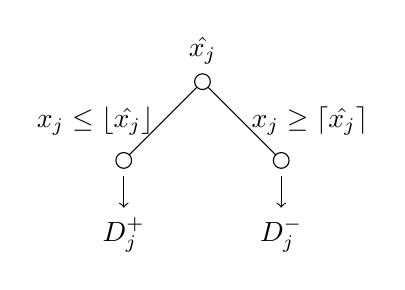
\begin{tikzpicture}[scale=0.2]
						\draw (0, 5) circle [radius=0.5];
						\draw (-5, 0) circle [radius=0.5];
						\draw (5, 0) circle [radius=0.5];
						\draw (0.353, 4.647) -- (4.647, 0.353);
						\draw (-0.353, 4.647) -- (-4.647, 0.353);
						\node [above] at (0, 5.5) {$\hat{x_j}$};
						\node [left] at (-2.5, 2.5) {$x_j \le \lfloor \hat{x_j} \rfloor$};
						\node [right] at (2.5, 2.5) {$x_j \ge \lceil \hat{x_j} \rceil$};
						\draw [->] (-5, -1) -- (-5, -3);
						\draw [->] (5, -1) -- (5, -3);
						\node [below] at (-5, -3) {$D_j^+$};
						\node [below] at (5, -3) {$D_j^-$};
					\end{tikzpicture}
					\caption{Strong Branching}
				\end{figure}
			
			\subsection{pseudo-cost Branching}
				Pseudo-cost is an estimate of per-unit change in the objective function, for each variable
				\begin{equation}\begin{cases}P_j^+, & \text{bound reduction if rounded up} \\ P_j^-, & \text{bound reduction if rounded down}\end{cases}\end{equation}
				define $f_j = x_j -\lfloor x_j \rfloor$
				\begin{equation}\begin{cases}D_j^+ = P_j^+ (1-f_j) \\ D_j^- = P_j^- f_j\end{cases}\end{equation}
		
		\section{Choose the Node to Branch}
			\subsection{Update After Branching}
				For those variables in $K$ find the \\
				- $\max \{\min\{ {D_j^+},  {D_j^-}\}\}$, or\\
				- $\max \{\max\{ {D_j^+},  {D_j^-}\}\}$, or\\
				- $\max \{\frac{D_j^+ + D_j^-}{2}\}$, or\\
				- $\max \{\alpha_1\min\{ {D_j^+},  {D_j^-}\} + \alpha_2\max\{ {D_j^+},  {D_j^-}\}\}$\\
				to branch.
		
			\subsection{Branch on Important Variables First}
				Branch on variables that affects many decisions.

			\subsection{Some Search Strategy}
				- Best Bound First: select the node with the largest bound (good for closing the gap)\\
				- Deep First: Good for finding Lower bound and easier to do dual simplex\\
				- Mix: Start with \lq\lq{}Deep First\rq\rq{} until we find a good bound and do \lq\lq{}Best Bound First\rq\rq{}

		\section{Types of Branching}
			\subsection{Traditional Branching}
				For $\hat{x} \notin S$, $\exists j \in N$ such that
				\begin{equation}\hat{x_j} -\lfloor\hat{x_j}\rfloor > 0 \end{equation}
				Create two sub-problems
				\begin{figure}[h!]
					\centering
					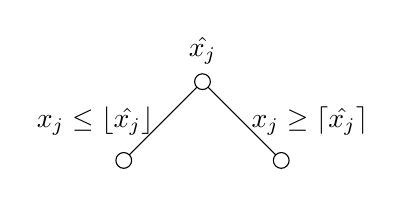
\begin{tikzpicture}[scale=0.2]
						\draw (0, 5) circle [radius=0.5];
						\draw (-5, 0) circle [radius=0.5];
						\draw (5, 0) circle [radius=0.5];
						\draw (0.353, 4.647) -- (4.647, 0.353);
						\draw (-0.353, 4.647) -- (-4.647, 0.353);
						\node [above] at (0, 5.5) {$\hat{x_j}$};
						\node [left] at (-2.5, 2.5) {$x_j \le \lfloor \hat{x_j} \rfloor$};
						\node [right] at (2.5, 2.5) {$x_j \ge \lceil \hat{x_j} \rceil$};
					\end{tikzpicture}
					\caption{Traditional Branching}
				\end{figure}

			\subsection{Constraint Branching}
				Use parallel constraints to branch, e.g.
				\begin{figure}[h!]
					\centering
					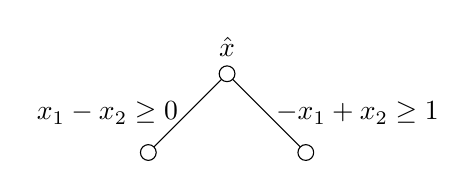
\begin{tikzpicture}[scale=0.2]
						\draw (0, 5) circle [radius=0.5];
						\draw (-5, 0) circle [radius=0.5];
						\draw (5, 0) circle [radius=0.5];
						\draw (0.353, 4.647) -- (4.647, 0.353);
						\draw (-0.353, 4.647) -- (-4.647, 0.353);
						\node [above] at (0, 5.5) {$\hat{x}$};
						\node [left] at (-2.5, 2.5) {$x_1 - x_2 \ge 0$};
						\node [right] at (2.5, 2.5) {$-x_1 + x_2 \ge 1$};
					\end{tikzpicture}
					\caption{Traditional Branching}
				\end{figure}
			
			\subsection{SOS}
				For SOS1,
				\begin{figure}[h!]
					\centering
					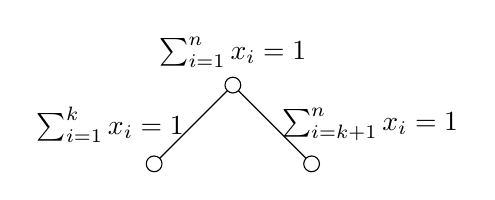
\begin{tikzpicture}[scale=0.2]
						\draw (0, 5) circle [radius=0.5];
						\draw (-5, 0) circle [radius=0.5];
						\draw (5, 0) circle [radius=0.5];
						\draw (0.353, 4.647) -- (4.647, 0.353);
						\draw (-0.353, 4.647) -- (-4.647, 0.353);
						\node [above] at (0, 5.5) {$\sum_{i=1}^{n}x_i=1$};
						\node [left] at (-2.5, 2.5) {$\sum_{i=1}^{k}x_i=1$};
						\node [right] at (2.5, 2.5) {$\sum_{i=k+1}^{n}x_i=1$};
					\end{tikzpicture}
					\caption{Traditional Branching}
				\end{figure}\\		
				For SOS2 (using the first definition),
				\begin{figure}[h!]
					\centering
					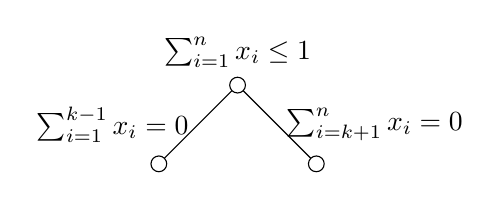
\begin{tikzpicture}[scale=0.2]
						\draw (0, 5) circle [radius=0.5];
						\draw (-5, 0) circle [radius=0.5];
						\draw (5, 0) circle [radius=0.5];
						\draw (0.353, 4.647) -- (4.647, 0.353);
						\draw (-0.353, 4.647) -- (-4.647, 0.353);
						\node [above] at (0, 5.5) {$\sum_{i=1}^{n}x_i \le 1$};
						\node [left] at (-2.5, 2.5) {$\sum_{i=1}^{k-1}x_i = 0$};
						\node [right] at (2.5, 2.5) {$\sum_{i=k+1}^{n}x_i =  0$};
					\end{tikzpicture}
					\caption{Traditional Branching}
				\end{figure}
			
			\subsection{GUB}
				This is where $x_i \in \{0, 1\}$, at most one variable can be 1,
				\begin{figure}[h!]
					\centering
					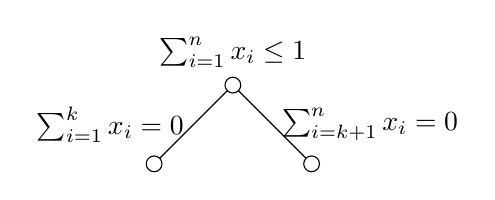
\begin{tikzpicture}[scale=0.2]
						\draw (0, 5) circle [radius=0.5];
						\draw (-5, 0) circle [radius=0.5];
						\draw (5, 0) circle [radius=0.5];
						\draw (0.353, 4.647) -- (4.647, 0.353);
						\draw (-0.353, 4.647) -- (-4.647, 0.353);
						\node [above] at (0, 5.5) {$\sum_{i=1}^{n}x_i\le 1$};
						\node [left] at (-2.5, 2.5) {$\sum_{i=1}^{k}x_i=0$};
						\node [right] at (2.5, 2.5) {$\sum_{i=k+1}^{n}x_i=0$};
					\end{tikzpicture}
					\caption{Traditional Branching}
				\end{figure}
			
			\subsection{Ryan-Foster}
				Ryan-Foster is for Set covering problem. The typical model is
				\begin{align}
					\text{min} \quad & \sum_{i \in C} x_i \\
					\text{s.t.} \quad & \sum_{i \in C} a_{ij}x_{i} \ge 1, \quad \forall j \in U \\
							& x_i \in \{0, 1\}, \quad \forall i \in C 
				\end{align}
				\textbf{Observation} For any fractional solution, there are at least two elements $(i,j)$ so that $i$ and $j$ are both partially covered by the same set $S$, but there is another set $T$ that only covers $i$
				\begin{figure}[h!]
					\centering
					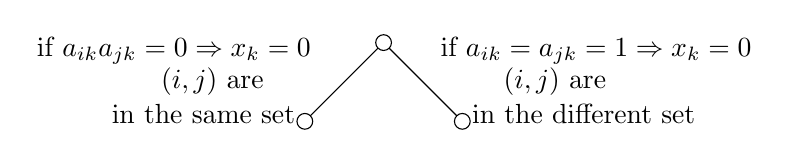
\begin{tikzpicture}[scale=0.2]
						\draw (0, 5) circle [radius=0.5];
						\draw (-5, 0) circle [radius=0.5];
						\draw (5, 0) circle [radius=0.5];
						\draw (0.353, 4.647) -- (4.647, 0.353);
						\draw (-0.353, 4.647) -- (-4.647, 0.353);
						\node [left] at (-7, 2.5) {$(i,j)$ are};
						\node [left] at (-5, 0.5) { in the same set};
						\node [left] at (-4, 4.5) {if $a_{ik}a_{jk}=0 \Rightarrow x_k = 0$};
						\node [right] at (7, 2.5) {$(i,j)$ are};
						\node [right] at (5, 0.5) { in the different set};
						\node [right] at (3, 4.5) {if $a_{ik}=a_{jk}=1 \Rightarrow x_k=0$};
					\end{tikzpicture}
					\caption{Traditional Branching}
				\end{figure}

	\chapter{Branch and Cut}
		\section{Separation Algorithm}
			Basic idea is to separate the feasible region so that the current "solution" (which is an fractional solution) is not included in the feasible region.
			\subsection{Vertices Packing}
				The current solution is $\bar{x} \in [0,1]^n$, we have two options to do the separation:\\
				\textbf{Option 1 - find the maximum clique:}\\
				(This approach is as hard as the original problem)\\
				denote
				\begin{equation}
					y_i=\begin{cases}1, \text{ if } i \in C \\ 0, \text{ otherwise}\end{cases}
				\end{equation}
				Find the maximum clique via:\\
				\begin{align}
					\max \quad &\sum \bar{x_i} y_i  \\
					\text{s.t.} \quad & y_i + y_j \le 1, \forall \{i, j\} \notin E 
				\end{align}\\
				\textbf{Option 2 - Heuristic:}\\
				\begin{algorithm}[h!]
					\caption{Heuristic method to find a clique}
					\begin{algorithmic}[1]
						\STATE find $v=\text{argmax}_{i\in V} \{\bar{x_i}\}, C=\{v\}$
						\WHILE {$u\in \text{argmax}_{i \in \cap_{i \notin C}N_{(i, j)}\notin C} \{\bar {x_1}\}$ exists}
							\STATE C.add(u)
						\ENDWHILE
						\STATE return C
					\end{algorithmic}
				\end{algorithm}\\
				If $\sum_{i\in C} \bar{x_i} > 1$ then add cut $\sum_{i\in C} x_i \le 1$

			\subsection{TSP}
				When we have a solution, i.e. $\bar{x}$, perform the sub-tour searching algorithm, if there exists any sub-tour, add the corresponded constraint. That is the separation.

		\section{Optional v.s. Essential Inequalities}
			\subsection{Valid (Optional) Inequalities}
				See Figure \ref{OptInq}
				\begin{figure}[!ht]
					\centering
					\begin{tikzpicture}[node distance = 2cm]
						\node (LR) [circleNode] {LR};
						\node (CG) [process, below of=LR] {Cut Generation};
						\node (CLimit) [decision, below of=CG] {Generated?};
						\node (Cont) [process, below of=CG, xshift=4cm] {Continue};
						\node (NLR) [circleNode, below of=CLimit] {New LR};
						\node (LNLR) [circleNode, below of=NLR, xshift=-2cm] {Branch 1};
						\node (RNLR) [circleNode, below of=NLR, xshift=2cm] {Branch 2};
						\draw [arrow] (LR) -- (CG);
						\draw [arrow] (CG) -- (CLimit);
						\draw [arrow] (CLimit) -- node [right] {yes} (NLR);
						\draw [arrow] (CLimit) -- node [below] {no} (Cont);
						\draw [arrow] (Cont) |- (CG);
						\draw [arrow] (NLR) -- (LNLR);
						\draw [arrow] (NLR) -- (RNLR);
					\end{tikzpicture}
					\caption {Branch and Cut for Optional Inequality}\label{OptInq}
				\end{figure}

			\subsection{Essential Inequalities (Lazy Cuts)}
				See Figure \ref{EssInq}
				\begin{figure}[!ht]
					\centering
					\begin{tikzpicture}[node distance = 1.8cm]
						\node (IS) [circleNode, label = above:integer solution] {IS};
						\node (CG) [process, below of=IS] {Cut Generation};
						\node (CLimit) [decision, below of=CG] {Generated?};
						\node (FI) [circleNode, below of=CLimit, label = below:feasible integer solution] {FI};
						\node (LP) [process, below of=CG, xshift = 3.5cm] {Solve Linear Relaxation};
						\node (LPF) [decision, below of=LP] {Feasible?};
						\node (NLR) [circleNode, below of=LPF] {New LR};
						\node (LNLR) [circleNode, below of=NLR, xshift=-2cm] {Branch 1};
						\node (RNLR) [circleNode, below of=NLR, xshift=2cm] {Branch 2};
						\node (Cont) [process, below of=LP, xshift=2.5cm] {Continue};
						\draw [arrow] (IS) -- (CG);
						\draw [arrow] (CG) -- (CLimit);
						\draw [arrow] (CLimit) -- node [right] {no} (FI);
						\draw [arrow] (CLimit) -- node [below] {yes} (LP);
						\draw [arrow] (LP) -- (LPF);
						\draw [arrow] (LPF) -- node [right] {no} (NLR);
						\draw [arrow] (LPF) -- node [below] {yes} (Cont);
						\draw [arrow] (NLR) -- (LNLR);
						\draw [arrow] (NLR) -- (RNLR);
						\draw [arrow] (Cont) |- (CG);
					\end{tikzpicture}
					\caption {Branch and Cut for Essential Inequality}\label{EssInq}
				\end{figure}

		\section{Chvatal-Gomory Cut}
			\subsection{Chvatal-Gomory Rounding Procedure}
				For $x=P\cap \mathbb{Z}_+^n$, where $P=\{x\in \mathbb{R}_+^n|Ax \le b\}$, A is an mxn matrix with columns $\{a_1, ..., a_n\}$ and $u \in \mathbb{R}_+^n$\\
				- The inequality
				\begin{equation}
					\sum_{j=1}^n ua_jx_j\le ub 
				\end{equation}
				is valid\\
				- Therefore the inequality
				\begin{equation}
					\sum_{j=1}^n \lfloor ua_j \rfloor x_j \le ub 
				\end{equation}
				is valid\\
				- Furthermore, the inequality
				\begin{equation}
					\sum_{j=1}^n \lfloor ua_j \rfloor x_j \le \lfloor ub \rfloor 
				\end{equation}
				is valid.

			\subsection{Gomory Cutting Plane}
				For a IP problem
				\begin{align}
					\max \quad & cx  \\
					\text{s.t.} \quad & Ax=b  \\
						& x \in \mathbb{B}^n 
				\end{align}
				let $\bar{x}$ be an optimal basic solution for the LR of P.
				\begin{equation}
					\bar{x} = \left[\begin{matrix} B^{-1}b \\ 0 \end{matrix}\right] = \left[ \begin{matrix}x_B \\ x_N\end{matrix}\right] 
				\end{equation}
				We have
				\begin{align}
					& Bx_B + Nx_N = b \\
					\Rightarrow \quad & x_B + B^{-1}Nx_N=B^{-1}b  \\
					\Rightarrow \quad & x_B + [\bar{a}_1, \bar{a}_2, ...]x_N = \bar{b} \\
					\Rightarrow \quad & x_i + \sum_{j\in NB} \bar{a}_{ij}x_j = \bar{b}_i \quad \text{(for the $i$th row)} 
				\end{align}
				Assume that $x_i \in \{0, 1\}$, use CG-Procedure
				\begin{equation}
					x_i + \sum_{j \in NB} \lfloor \bar{a}_{ij} \rfloor x_j \le \lfloor \bar{b}_i \rfloor 
				\end{equation}
				is a valid constraint for $P$, furthermore,
				\begin{equation}
					(\bar{b}_i - \sum_{j\in NB} \bar{a}_{ij}x_j) + \sum_{j\in NB}\lfloor \bar{a}_{ij} \rfloor x_j\le \lfloor \bar{b}_i \rfloor 
				\end{equation}
				Move the item, we get a new Gomory Cutting Plane
				\begin{equation}
					\sum_{j\in NB} (\bar{a}_{ij} - \lfloor \bar{a}_{ij} \rfloor)x_j \ge \bar{b}_i - \lfloor \bar{b}_i \rfloor  
				\end{equation}
				Add this inequality to the LR, use the dual simplex method to do one pivot, we get a new solution. Use Gomory cutting plane iteratively and we can find the optimal solution for IP.

	\chapter{Typical IP problems}
		\section{Packing and Matching}
			\subsection{Vertices Packing Formulation}
				Given a graph $G=(V, E)$, with $|V|=n$. A vertices packing solution is that no two neighboring vertices can be chosen at the same time.
				\begin{equation}
					PACK(G) = \{x\in \mathbb{B}^n|x_i + x_j \le 1, \forall (i, j)\in E\} 
				\end{equation}
				\framebox{\textbf{Example:}}
				\begin{figure}[!ht]
					\centering
					\begin{tikzpicture}[node distance = 1.8cm]
						\node (1) [circleNode] {1};
						\node (2) [circleNode, below of=1] {2};
						\node (3) [circleNode, below of=2, xshift=-2cm] {3};
						\node (4) [circleNode, below of=2, xshift=2cm] {4};
						\draw (1) -- (2);
						\draw (1) -- (3);
						\draw (1) -- (4);
						\draw (2) -- (4);
						\draw (3) -- (4);
					\end{tikzpicture}
					\caption{Example of vertices packing problem}
				\end{figure}
				The PACK of this graph is\\
				\begin{equation}
					PACK = conv\left(
						\left(\begin{matrix}0 \\ 0 \\ 0 \\ 0\end{matrix}\right),
						\left(\begin{matrix}1 \\ 0 \\ 0 \\ 0\end{matrix}\right),
						\left(\begin{matrix}0 \\ 1 \\ 0 \\ 0\end{matrix}\right),
						\left(\begin{matrix}0 \\ 0 \\ 1 \\ 0\end{matrix}\right),
						\left(\begin{matrix}0 \\ 0 \\ 0 \\ 1\end{matrix}\right),
						\left(\begin{matrix}0 \\ 1 \\ 1 \\ 0\end{matrix}\right)
						\right)
				\end{equation}

			\subsection{Matching Formulation}
				Given a graph $G=(V, E)$, denote $\delta(i)$ as the set of all the edges introduced to vertice $i\in V$. A matching solution is that no two edges introduced to the same vertice can be chosen at the same time.
				\begin{equation}
					MATCH(G) = \{\sum_{e\in \delta(i)}x_e \le 1|i\in V\}
				\end{equation}

			\subsection{Dimension of PACK(G)}
				The dimension of PACK, i.e. $dim(PACK(G))$ is (full-dimensional)
				\begin{equation}
					dim(PACK(G)) = |V| 
				\end{equation}
				To prove that $dim(PACK(G)) = |V|$, we need to find $|V| + 1$ affinely independent vectors.\\
				\framebox{\textbf{Proof:}}\\
					\begin{equation}
						rank\left(\left[\begin{matrix}0 & I_{|V|} \\ 1 & 1\end{matrix}\right]\right) = |V| + 1 
					\end{equation}
				Therefore, in PACK, $rank(A^=,b^=)=0$ 
			
			\subsection{Clique}
				- A \textbf{clique} is a subset of a graph that in the clique every two vertices linked with each other (complete sub-graph).
				- A \textbf{maximum clique} is a clique that any other vertice can not form a clique with all the points in this clique.

			\subsection{Inequalities and Facets of conv(VP)}
				\framebox{\textbf{Example:}}\\
					\begin{figure}[!ht]
						\centering
						\begin{tikzpicture}[node distance = 1.2cm]
							\node (1) [circleNode] {1};
							\node (2) [circleNode, below of=1, xshift=-2cm] {2};
							\node (3) [circleNode, below of=1, xshift=2cm] {3};
							\node (4) [circleNode, below of=2, xshift=2cm] {4};
							\node (5) [circleNode, below of=4, xshift=-0.9cm] {5};
							\node (6) [circleNode, below of=4, xshift=0.9cm] {6};
							\draw (1) -- (2);
							\draw (1) -- (3);
							\draw (1) -- (4);
							\draw (3) -- (4);
							\draw (2) -- (5);
							\draw (5) -- (6);
							\draw (6) -- (3);
						\end{tikzpicture}
						\caption{Example}
					\end{figure}

				\subsubsection{Type 1 (Nonnegative Constraints)}
					$x_i \ge 0$ induce facets.\\
					\framebox{\textbf{Proof:}}
					\begin{equation}
						rank\left(\left[\begin{matrix}0 & 0 \\ 0 & I_{|V|}\end{matrix}\right]\right) = |V| + 1 
					\end{equation}

				\subsubsection{Type 2 (Neighborhood Constraints)}
					$x_i + x_j \le 1$ is a valid constraint, but it \textbf{DOES NOT} always induce facet.

				\subsubsection{Type 3 (Odd Hole)}
					$H$ is an odd hole if it contains circle of $k$ nodes, such that $k$ is odd and there is no cords. e.g. \{1, 2, 5, 6, 3\}. Then, the following inequality is valid,
					\begin{equation}
						\sum_{i\in H}x_i\le \frac{|H|-1}2 
					\end{equation}
					Odd Hole inequality \textbf{DOES NOT} always induce facets.\\
					This inequality can be derived from Gomory cut.

				\subsubsection{Type 4 (Maximum Clique)}
					$C$ is a maximum clique, then the following inequality is valid and induce a facet,
					\begin{equation}
						\sum_{i\in C} x_i \le 1 
					\end{equation}
					\framebox{\textbf{Proof:}}\\
						First, if $C=V$
						\begin{equation}
							rank\left(\left[I\right]\right) = |C| = |V| 			
						\end{equation}
						Second, if $C$ is a subset of $V$, for each vertice in $V \setminus C$, there should be at least one vertice in $C$ that is not linked with it. Therefore for each vertice in $C$ we can find a packing.

			\subsection{Gomory Cut in Set Covering}
				Consider a graph $G=(V, E)$, the covering problem is
				\begin{equation}
					\sum_{e\in \delta(i)}x_e \le 1, i\in V, x_e\in \{0, 1\}, e\in E
				\end{equation}
				For $T\subset V$, denote $\delta(i)$ as all edges induce to $i\in V$, denote $E(T) \subset E$ as all the edges linked between $(i, j), i\in T, j\in T$, therefore we have
				\begin{equation}
					\sum_{i\in T}\sum_{e\in \delta(i)}x_e \le |T| 
				\end{equation}
				For edges linking $i \in T, j \in T$, count them twice, for edges linking $i\in T, j\notin T$, count them once.We can have a new constraint
				\begin{equation}
					2\sum_{e\in E(T)}x_e + \sum_{e\in \delta(V\setminus T, T)}x_e \le |T| 
				\end{equation}
				Perform the Gomory Cut, the following constraint is a valid:
				\begin{equation}
					\sum_{e\in E(T)}x_e \le \lfloor \frac{|T|}2 \rfloor 
				\end{equation}
							
		\section{Traveling Salesman Problem}
			\subsection{TSP Formulation (Asymmetric)}
				Consider a Graph $G=\{A, N\}$\\
				Denote:\\
				\begin{equation}
					x_{ij} = \begin{cases}1, &\text{if goes from } i \text{ to } j\\ 0, & \text{otherwise}\end{cases}
				\end{equation}
				\textbf{Dantzig-Fulkerson-Johnson Formulation:}
				\begin{align}
					\min &\sum_{(i, j)\in A} c_{ij}x_{ij} \\
					& \sum_{j \in N, (i,j)\in A} x_{ij} = 1 \\
					& \sum_{i \in N, (i,j)\in A} x_{ij} = 1 \\
					& \sum_{j\notin S, i\in S, (i,j)\in A} x_{ij} = 1\text{ or } \sum_{i, j \in S, (i, j) \in A} x_{ij} \le |S| - 1 \\
					& \forall S \subset N, S\ne \emptyset, 2\le |S| \le n-1 
				\end{align}
				\textbf{Miller-Tucker-Zemlin Formulation:}
				\begin{align}
					\min &\sum_{(i, j)\in A} c_{ij}x_{ij} \\
					& \sum_{j \in N, (i,j)\in A} x_ij = 1 \\
					& \sum_{i \in N, (i,j)\in A} x_ij = 1 \\
					& u_i - u_j +nx_{ij}\le n-1 \quad i, j\in{2, ... , n}, (i, j)\in A \\
					& u_1 = 1 \\
					& 2 \le u_i \le n, i\in N, i>1 
				\end{align}

			\subsection{Sub-tour Searching Algorithm}
				In the graph $G=(N, A)$, let $\bar{G}=(N, \bar{A})$ be the connected components of graph, where
				\begin{equation}\bar{G}=(G, \bar{A}), \bar{A}=\{(i, j) \in A | \bar{x_{ij}}=1\} \end{equation}
				denote
				\begin{equation}\bar{FS}(i) = \{(i,j)\in \bar{A}\} \end{equation}
				Then the algorithm to find all sub-tour is the following:
				\begin{algorithm}[h!]
					\caption{Sub-tour Searching Algorithm}
					\begin{algorithmic}[1]
						\STATE $K = \emptyset$
						\STATE $d_i = 0, \forall i \in N$
						\FOR {$i\in N$}
							\STATE $C = \emptyset$
							\STATE $Q = \emptyset$
							\IF {$d_i == 0$}
								\STATE $d_i = 1$
								\STATE $C = C\cup \{i\}$
								\STATE Q.append(i)
								\WHILE {$Q\ne \emptyset$}
									\STATE v = Q.pop()
									\FOR {$u \in \bar{FS}(v)$}
										\IF {$d_u == 0$}
											\STATE $d_u = 1$
											\STATE $C = C \cup \{u\}$
											\STATE Q.append(u)
										\ENDIF
									\ENDFOR
								\ENDWHILE
							\ENDIF
							\STATE $K=K\cup C$
						\ENDFOR
					\end{algorithmic}
				\end{algorithm}
			
		\section{Knapsack Problem}
			\subsection{Knapsack Problem Formulation}
				Consider the knapsack set KNAP
				\begin{equation}conv(KNAP)= conv(\{x\in \mathbb{B}^n|\sum_{j\in N}a_jx_j\le b\})\end{equation}
				in where\\
				- $N = \{1, 2, ..., n\}$\\
				- With out lost of generality, assume that $a_j > 0, \forall j \in N$ and $a_j < b, \forall j \in N$

			\subsection{Valid Inequalities for a Relaxation}
				For $P=\{x\in \mathbb{B}^n | Ax\le b\}$, each row can be regard as a Knapsack problem, i.e. for row $i$
				\begin{equation}
					P_i = \{x\in \mathbb{B}^n | a_i^T x \le b_i\} 
				\end{equation}
				is a relaxation of $P$, therefore,
				\begin{equation}
					P\subseteq P_i, \forall i=1,2,...,m 
				\end{equation}
				\begin{equation}
					P\subseteq \cap_{i=1}^m P_i 
				\end{equation}
				So any inequality valid for a relaxation of an IP is also valid for IP itself.
				
			\subsection{Cover and Extended Cover}
				A set $C\subseteq N$ is a cover if $\sum_{j\in C} a_j > b$, a cover $C$ is minimal cover if
				\begin{equation}
					C\subseteq N | \sum_{j\in C}a_j>b, \sum_{j\in C\setminus k} a_j < b, \forall k \in C 
				\end{equation}
				For a cover $C$, we can have the cover inequality
				\begin{equation}
					\sum_{j\in C}x_j \le |C|-1
				\end{equation}
				The inequality is trivial considering the pigeonhole principle.\\
				$C\subseteq N$ is a minimal cover, then $E(C)$ is defined as following:
				\begin{equation}
					E(C) = C\cup \{j \in N | a_j \ge a_i, \forall i \in C\}
				\end{equation}
				is called an extended cover. Then we have,
				\begin{equation}
					\sum_{i\in E(C)} x_i \le |C| - 1 \text{ dominates } \sum_{i\in C} x_i \le |C| - 1
				\end{equation}
				and
				\begin{equation}
					\sum_{i\in E(C)} x_i \le |C| - 1 \text{ dominates } \sum_{i\in E(C)} x_i \le |E(C)| - 1
				\end{equation}
				Hereby we need to prove that $\sum_{i\in E(C)} x_i \le |C| - 1$ is valid, by contradiction.\\
				\framebox{\textbf{Proof:???}} Suppose $x^R \in KNAP$, $R$ is a feasible solution, Where
				\begin{equation}
					x^R_j = \begin{cases}1, \quad \text{if $j\in R$} \\ 0, \quad \text{otherwise}\end{cases} 
				\end{equation}
				Then
				\begin{equation}
					\sum_{j\in E(C)}x^R_j \ge |C| \Rightarrow |R \cap E(C)| \ge |C|  
				\end{equation}
				therefore
				\begin{equation}
					\sum_{j\in R}a_j \ge \sum_{j\in R \cap E(C)} a_j \ge \sum_{j\in C} a_j > b 
				\end{equation}
				which means $R$ is a cover, it is contradict to $\sum_{j\in E(C)}x^R_j \ge |C|$ so $x^R \notin KNAP$

			\subsection{Dimension of KNAP}
				$conv(KNAP)$ is full dimension, i.e. $dim(conv(KNAP))=n$.\\
				\framebox{\textbf{Proof:}} $0, e_j, \forall j\in N$ are $n + 1$ affinely independent points in $conv(KNAP)$\\

			\subsection{Inequalities and Facets of conv(KNAP)}
				\subsubsection{Type 1 (Lower Bound and Upper Bound Constraints):}
					- $x_k\ge 0$ is a facet of $conv(KNAP)$\\
					\framebox{\textbf{Proof:}} $0, e_j, \forall j\in N\setminus k$ are $n$ affinely independent points that satisfied $x_k=0$\\
					- $x_k\le 1$ is a facet iff $a_j + a_k \le b, \forall j\in N \setminus k$\\
					\framebox{\textbf{Proof:}} $e_k, e_j+e_k, \forall j \in N\setminus k$ are $n$ affinely independent points that satisfied $x_k = 1$

				\subsubsection{Type 2 (Extended Cover)}
					Order the variables so that $a_1 \ge a_2 \ge \dots \ge a_n$, therefore $a_1 = a_{max}$\\
					Let $C$ be a cover with $\{j_1, j_2, \dots, j_r\}$ where $j_1 < j_2 < \dots < j_r$ so that $a_{j_1} \ge a_{j_2} \ge \dots \ge a_{j_r}$\\
					Let $p = \min\{j | j\in N \setminus E(C)\}$\\
					Then
					\begin{equation}
						\sum_{j\in E(C)} x_j \le |C| - 1 
					\end{equation}
					is a facet of $conv(KNAP)$ if\\
					- $C = N$\\
					\framebox{\textbf{Proof:}}
					\begin{equation}
						R_k = C\setminus k, \forall k \in C = N \setminus k, \forall k \in N 
					\end{equation}
					have $|N|$ affinely independent vectors\\
					- $E(C) = N$ and $\sum_{j\in C \setminus \{j_1, j_2\}} a_j + a_{max} \le b$\\
					\framebox{\textbf{Proof:}} ($j_1, j_2$ are two heaviest elements in $C$)
					\begin{equation}
						S_k = C\setminus \{j_1, j_2\}\cup \{k\}, \forall k\in E(C)\setminus C 
					\end{equation}
					$R_k\cup S_k$ have $|C|+|E(C) \setminus C| = |E(C)| = |N|$ affinely independent vectors\\
					- $C = E(C)$ and $\sum_{j\in C \setminus j_1} a_j + a_p \le b$)\\
					\framebox{\textbf{Proof:}} ($j_1$ is the heaviest element in $C$, $k$ is the lightest element outside extended cover)
					\begin{equation}
						T_k = C \setminus j_i \cup \{k\}, \forall k\in N\setminus E(C) 
					\end{equation}
					$R_k \cup T_k$ have $|N \setminus E(C)| + |E(C)| = |N\setminus C| + |C| = |N|$ affinely independent vectors\\
					- $C \subset E(C) \subset N$ and $\sum_{j\in C \setminus \{j_1, j_2\}} a_j + a_{max} \le b$ and $\sum_{j\in C \setminus j_1} a_j + a_p \le b$\\
					\framebox{\textbf{Proof:}}$S_k \cup T_k$ have $|E(C) \setminus C| + |N \setminus E(C)| = |N|$ affinely independent vectors

			\subsection{Lifting}
				\subsubsection{Up Lifting}
					For KNAP problem
					\begin{equation}
						KNAP = \{x\in \mathbb{B}^n | \sum_j a_jx_j \le b\} 
					\end{equation}
					For $P=conv(KNAP)$ denote\\
					\begin{align}
						&P_{k_1, k_2, ..., k_m} \\
						&\quad =conv(KNAP\cap \{x\in \mathbb{B}^{n}|x_{k_1}=x_{k_2}=\dots=x_{k_m}=0\}) 
					\end{align}
					Therefore
					\begin{align}
						&P_{k_1, k_2, ..., k_m} \\
						&\quad=conv(KNAP\cap \{x\in \mathbb{B}^{n}|\sum_{j\in N\setminus \{k_1, k_2, ..., k_m\}} a_j x_j \le b\}) 
					\end{align}
					The $C=N$ cover inequality for $P_{k_1, k_2, ..., k_m}$ implies
					\begin{equation}
						\sum_{j\in N\setminus \{k_1, k_2, ..., k_m\}} x_j \le n-m-1 
					\end{equation}
					is a facet of $P_{k_1, k_2, ..., k_m}$\\
					The lifting process is to find a facet for $P_{k_1, k_2, ..., k_{m-1}}$ using facet of $P_{k_1, k_2, ..., k_m}$, i.e. find $\alpha_{m}$ for the following constraint to be a facet.
					\begin{equation}
						\alpha_m x_m + \sum_{j\in N\setminus \{k_1, k_2, ..., k_m\}} x_j \le n-m-1 
					\end{equation}
					If $x_m=0$, $\alpha_m \ge 0$,\\
					If $x_m=1$, $\alpha_m \le (n-m+1) - \gamma$ where
					\begin{align}
						\gamma &= \max\{\sum_{j\in N\setminus\{k_1, k_2, ..., k_m\}}x_j|x\in P_{k_1, k_2, ..., k_{m-1}}, x_m=1\} \\
						&= \max\{\sum_{j\in N\setminus\{k_1, k_2, ..., k_m\}}x_j|\sum_{j \in N \setminus \{k_1, k_2, ..., k_m\}}a_jx_j\le b-a_m\} 
					\end{align}
					Then let $\alpha_m = n-m+1-\gamma$, we uplifted a constraint. Repeat this procedure for $\{k_1, k_2, ..., k_m\}$ and finally we can find a family of facets for $conv(KNAP)$


				\subsubsection{Down Lifting}
					Similar to up lifting, we can perform the lifting in a different way.\\
					Denote
					\begin{align}
						&P_{k_1, k_2, ..., k_m}^{'} \\
						&\quad =conv(KNAP\cap \{x\in \mathbb{B}^{n}|x_{k_1}=x_{k_2}=\dots=x_{k_m}=1\}) 
					\end{align}

			\subsection{Separation of a Cover Inequality}
				$C\in N$ is a cover if $\sum_{i\in C} a_i > b$, let $C$ be a minimal cover
				\begin{align}
					&\sum_{i\in C}x_i \le |C| - 1 \\
					\Rightarrow \quad & |C| - \sum_{i\in C}x_i = \sum_{i \in C}(1-x_i)\ge 1 \\
				\end{align}
				let $\bar{x}$ be a fractional solution of $\{\sum_{i\in N} a_ix_i \le b, x_i \in [0, 1], i\in N\}$, find a cover $C$ of which $\sum_{i\in C}(1-\bar{x_i})<1$\\
				Decision variable:
				\begin{equation}
					y_i = \begin{cases}1, \quad \text{if } i\in C\\ 0, \quad \text{otherwise}\end{cases}
				\end{equation}
				\begin{align}
					\min \quad & \sum_{i\in N} (1-\bar{x_i})y_i = z \\
					\text{s.t.} \quad & \sum_{i\in N}a_iy_i \ge b+1 \\
					&y_i \in \{0, 1\}, i\in N
				\end{align}
				if $z<1$, then the cover cut associated with $y$ is violation by $\bar{x}$

		\section{Network Flow Problem}
			(Network Flow Problem is a special type of IP problem, its linear relaxation is the convex hull of the original problem.)
			\subsection{Shortest Path Problem}
				A graph $G=(A, N)$ is a directed graph\\
				\begin{figure}[!ht]
					\centering
					\begin{tikzpicture}[node distance = 1.8cm]
						\node (1) [circleNode, label=above:start] {1};
						\node (2) [circleNode, right of=1, yshift=1cm] {2};
						\node (3) [circleNode, right of=1, yshift=-1cm] {3};
						\node (4) [circleNode, right of=2] {4};
						\node (5) [circleNode, right of=3] {5};
						\node (6) [circleNode, label=above:end, right of=4, yshift=-1cm] {6};
						\draw [arrow] (1) -- (2);
						\draw [arrow] (1) -- (3);
						\draw [arrow] (2) -- (3);
						\draw [arrow] (2) -- (4);
						\draw [arrow] (3) -- (5);
						\draw [arrow] (4) -- (6);
						\draw [arrow] (5) -- (6);
						\draw [arrow] (5) -- (4);
						\draw [arrow] (2) -- (5);
					\end{tikzpicture}
					\caption{Example of directed graph}
				\end{figure}
				Denote:\\
				\begin{equation}
					x_{ij} = \begin{cases}1, &\text{if goes from } i \text{ to } j\\ 0, & \text{otherwise}\end{cases}
				\end{equation}
				The shortest path problem can be formulated as the following:\\
				\begin{align}
					\min &\sum_{(i, j)\in A} c_{ij}x_{ij} \\
					& \sum_{i \in N\setminus(\{S\}\cup\{E\}), (i,j)\in A} x_{ij} - \sum_{j \in N, (i,j)\in A} x_{ji} = 0 \\
					& \sum_{i=\{S\}, (i,j)\in A} x_{ij} - \sum_{j \in N, (i,j)\in A} x_{ji} = 1 \\
					& \sum_{i=\{E\}, (i,j)\in A} x_{ij} - \sum_{j \in N, (i,j)\in A} x_{ji} = -1 \\
					& x_{ij} \in [0,1], (i,j)\in A 
				\end{align}
				Although initially $x_{ij} \in [0,1]$, in the optimized solution, $x\in \{0, 1\}$.

			\subsection{Maximum Flow Problem}
				\begin{align}
					\min &\sum_{(i, j)\in A} F \\
					& \sum_{i \in N\setminus(\{S\}\cup\{E\}), (i,j)\in A} x_{ij} - \sum_{j \in N, (i,j)\in A} x_{ji} = 0 \\
					& \sum_{i=\{S\}, (i,j)\in A} x_{ij} - \sum_{j \in N, (i,j)\in A} x_{ji} = F \\
					& \sum_{i=\{E\}, (i,j)\in A} x_{ij} - \sum_{j \in N, (i,j)\in A} x_{ji} = -F \\
					& l_{ij} \le x_{ij} \le u_{ij}, (i,j)\in A 
				\end{align}
				In where $F$ means the flow from source to target.

			\subsection{Minimum Cost Flow}
				The shortest path problem is a special case of Minimum Cost Flow Problem, which can be formulated as the following:\\
				\begin{align}
					\min &\sum_{(i, j)\in A} c_{ij}x_{ij} \\
					& \sum_{i \in N\setminus(\{S\}\cup\{E\}), (i,j)\in A} x_{ij} - \sum_{j \in N, (i,j)\in A} x_{ji} = 0 \\
					& \sum_{i=\{S\}, (i,j)\in A} x_{ij} - \sum_{j \in N, (i,j)\in A} x_{ji} = 1 \\
					& \sum_{i=\{E\}, (i,j)\in A} x_{ij} - \sum_{j \in N, (i,j)\in A} x_{ji} = -1 \\
					& x_{ij} \in [0,1], (i,j)\in A 
				\end{align}				
			
			\subsection{Unimodularity}
				\subsubsection{Unimodular Matrix and Total Unimodular Matrix}
					- A unimodular matrix $M$ is a squared matrix, where $det(M)=1$ or $-1$.\\
					- Total unimodular matrix is a matrix where all its sub-matrices are unimodular matrix.

				\subsubsection{Importance of Unimodular Matrix}
					Let $M_{m\times m}$ be a unimodular matrix, if $b\in \mathbb{Z}^m$, the solution for $Mx=b$ is always integer.\\
					\framebox{\textbf{Proof:}} By Cramer's Rule
					\begin{equation}
						x_i = \frac{det{M_i}}{det{M}} 
					\end{equation}
					in which $M_i$ is matrix $M$ replace $i$th column with $b$. Therefore $det(M_i)$ is integer. Also, $det(M)\ne 0$, so $det(M)=1$ or $det(M)=-1$. Proved.

				\subsubsection{Structures of Total Unimodular Matrix}
					\textbf{Structure 1:}
						Matrix $M$ that has only 1, -1, 0 enters and each column has at most 2 non-zeros is a TU matrix if it satisfies the following conditions:\\
						We can split the rows in to tops and bottoms, such that for all columns $j$ having 2 non-zeros\\
						- If the non-zeros have the same sign, then one value should be in top and the other should be in bottom\\
						- If the non-zeros have the different sign, then both of them should be in top or both of them should be in bottom\\
					\textbf{Structure 2:}
						If all the columns in matrix $M$ has only 0 or consecutive 1s (or -1s), matrix $M$ is a TU matrix

				\subsubsection{Construct a New Unimodular Matrix}
					Let $F$ be a unimodular matrix, then
					\begin{equation}
						\left[\begin{matrix}F \\ I\end{matrix}\right] 
					\end{equation}
					is a unimodular matrix, also
					\begin{equation}
						\left[\begin{matrix}F & 0 \\ I & I\end{matrix}\right] 
					\end{equation}
					is a unimodular matrix.